\chapter{Circuits séquentiels}
\section{Introduction}
Contrairement aux CLC (circuits logiques combinatoires), les sorties des les circuits logiques séquentiels ne dépendent pas que des entrées.
\subsection{Exemple}
Considérons le problème suivant: «on souhaite contrôler à l’aide d’un système logique la vanne de remplissage d’un réservoir. Le réservoir
dispose de deux capteurs 1 et 2 permettant de détecter le niveau maximal et le niveau minimal dans le réservoir.»\\
\begin{minipage}[t]{.5\textwidth}
Le système devrait assurer que
le niveau dans le réservoir ne soit
jamais au dessus de niveau
indiqué par le capteur 1 ($c_1$),
ni en dessous de niveau
indiqué par le capteur 2 ($c_2$).
\end{minipage}
\begin{minipage}{.5\textwidth}
	\begin{figure}[H]
		\centering
		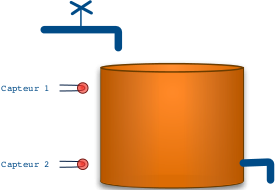
\includegraphics[width=.8\textwidth]{ch6/image1}
	\end{figure}
\end{minipage}
\ \\\\
Imaginons 2 situation:\\\\
\begin{minipage}{.5\textwidth}
	Réservoir plein en train de se vider:
	\begin{figure}[H]
		\centering
		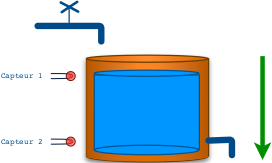
\includegraphics[width=.6\textwidth]{ch6/image2}
	\end{figure}
	\begin{table}[H]
		\centering
		$\begin{array}{c|c|c}
			$initial$ & $valeurs$ & $sortie$\\
			\hline
			\begin{array}{c}
				c_1=1\\
				c_2=1
			\end{array} & \begin{array}{c}
				c_1 = 0\\
				c_2=1
			\end{array} & 0
		\end{array}$
	\end{table}
\end{minipage}
\begin{minipage}{.5\textwidth}
	Réservoir vide en train de se remplir:
	\begin{figure}[H]
		\centering
		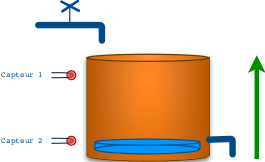
\includegraphics[width=.6\textwidth]{ch6/image3}
	\end{figure}
	\begin{table}[H]
		\centering
		$\begin{array}{c|c|c}
			$initial$ & $valeurs$ & $sortie$\\
			\hline
			\begin{array}{c}
				c_1=0\\
				c_2=0
			\end{array} & \begin{array}{c}
				c_1 = 0\\
				c_2=1
			\end{array} & 1
		\end{array}$
	\end{table}
\end{minipage}\ \\\\
Ainsi, pour une même combinaison d'entrées, nous avons 2 sorties!\\
Il nous faut mémoriser d'où est-ce que l'on vient $\Rightarrow$ notion d'état.
\subsection{Représentation avec les états}
\section{Systèmes séquentiels formellement}

\section{Représentation des systèmes séquentiels}
